\documentclass[sigchi]{acmart}

\usepackage{booktabs} % For formal tables


% Copyright
\setcopyright{none}
%\setcopyright{acmcopyright}
%\setcopyright{acmlicensed}
%\setcopyright{rightsretained}
%\setcopyright{usgov}
%\setcopyright{usgovmixed}
%\setcopyright{cagov}
%\setcopyright{licensedcagov}
%\setcopyright{cagovmixed}
%\setcopyright{licensedothergov}

% DOI
%\acmDOI{10.475/123_4}

% ISBN
%\acmISBN{123-4567-24-567/08/06}

%Conference
%\acmConference[WOODSTOCK'97]{ACM Woodstock conference}{July 1997}{El
% Paso, Texas USA}
%\acmYear{1997}
%\copyrightyear{2016}

%\acmPrice{15.00}


\begin{document}
\title{ConWearDi - Digitalisierung von Baudienstleistungen und -prozessen}
%\titlenote{Produces the permission block, and
%  copyright information}
\subtitle{Option einen Subtitel hinzuzufügen}
%\subtitlenote{The full version of the author's guide is available as \texttt{acmart.pdf} document}

\author{Ben Trovato}
\authornote{Dr.~Trovato insisted his name be first.}
\orcid{1234-5678-9012}
\affiliation{%
  \institution{Institute for Clarity in Documentation}
  \streetaddress{P.O. Box 1212}
  \city{Dublin}
  \state{Ohio}
  \postcode{43017-6221}
}
\email{trovato@corporation.com}

\author{G.K.M. Tobin}
\authornote{The secretary disavows any knowledge of this author's actions.}
\affiliation{%
  \institution{Institute for Clarity in Documentation}
  \streetaddress{P.O. Box 1212}
  \city{Dublin}
  \state{Ohio}
  \postcode{43017-6221}
}
\email{webmaster@marysville-ohio.com}

\author{Lars Th{\o}rv{\"a}ld}
\authornote{This author is the
  one who did all the really hard work.}
\affiliation{%
  \institution{The Th{\o}rv{\"a}ld Group}
  \streetaddress{1 Th{\o}rv{\"a}ld Circle}
  \city{Hekla}
  \country{Iceland}}
\email{larst@affiliation.org}

\author{Valerie B\'eranger}
\affiliation{%
  \institution{Inria Paris-Rocquencourt}
  \city{Rocquencourt}
  \country{France}
}
\author{Aparna Patel}
\affiliation{%
 \institution{Rajiv Gandhi University}
 \streetaddress{Rono-Hills}
 \city{Doimukh}
 \state{Arunachal Pradesh}
 \country{India}}
\author{Huifen Chan}
\affiliation{%
  \institution{Tsinghua University}
  \streetaddress{30 Shuangqing Rd}
  \city{Haidian Qu}
  \state{Beijing Shi}
  \country{China}}

\author{Charles Palmer}
\affiliation{%
  \institution{Palmer Research Laboratories}
  \streetaddress{8600 Datapoint Drive}
  \city{San Antonio}
  \state{Texas}
  \postcode{78229}}
\email{cpalmer@prl.com}

\author{John Smith}
\affiliation{\institution{The Th{\o}rv{\"a}ld Group}}
\email{jsmith@affiliation.org}

\author{Julius P.~Kumquat}
\affiliation{\institution{The Kumquat Consortium}}
\email{jpkumquat@consortium.net}

% The default list of authors is too long for headers.
\renewcommand{\shortauthors}{B. Trovato et al.}

\newcommand{\todo}[1]{\textcolor{red}{TODO: #1}}

\begin{abstract}
\todo{write short abstract or remove it completely}
\end{abstract}

%
% The code below should be generated by the tool at
% http://dl.acm.org/ccs.cfm
% Please copy and paste the code instead of the example below.
%
%\begin{CCSXML}
%<ccs2012>
% <concept>
%  <concept_id>10010520.10010553.10010562</concept_id>
%  <concept_desc>Computer systems organization~Embedded systems</concept_desc>
%  <concept_significance>500</concept_significance>
% </concept>
% <concept>
%  <concept_id>10010520.10010575.10010755</concept_id>
%  <concept_desc>Computer systems organization~Redundancy</concept_desc>
%  <concept_significance>300</concept_significance>
% </concept>
% <concept>
%  <concept_id>10010520.10010553.10010554</concept_id>
%  <concept_desc>Computer systems organization~Robotics</concept_desc>
%  <concept_significance>100</concept_significance>
% </concept>
% <concept>
%  <concept_id>10003033.10003083.10003095</concept_id>
%  <concept_desc>Networks~Network reliability</concept_desc>
%  <concept_significance>100</concept_significance>
% </concept>
%</ccs2012>
%\end{CCSXML}
%
%\ccsdesc[500]{Computer systems organization~Embedded systems}
%\ccsdesc[300]{Computer systems organization~Redundancy}
%\ccsdesc{Computer systems organization~Robotics}
%\ccsdesc[100]{Networks~Network reliability}
%

% \keywords{ACM proceedings, \LaTeX, text tagging}

\begin{teaserfigure}
  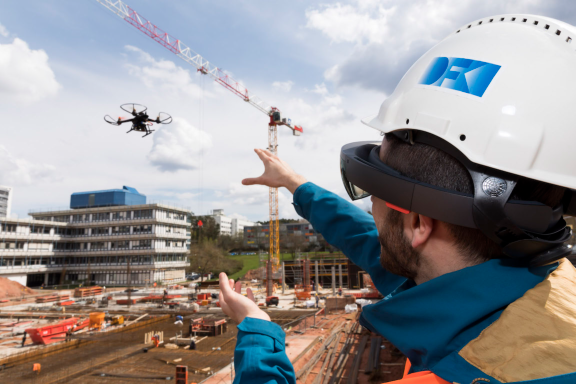
\includegraphics[width=\textwidth]{teaser}
  \caption{In the project's vision, construction workers have access to and can intuitively interact with digital information, e.g. plans, instructions, etc., meanwhile intelligent sensors capture the progress and state of the construction in real time. Photo: DFKI}
  \label{fig:teaser}
\end{teaserfigure}


\maketitle

\section{Introduction}
Considering active digitization projects, the construction industry seems yet a mostly unconquered field.
Complex dynamics and sometimes harsh (e.g. weather influence, no infrastructure, etc.) environments of construction sites challenge the technology and adds harder requirements compared to an industrial application on a shop floor. 
Moreover, the typically conservative and hierarchical work culture makes the introduction and acceptance of new methods more challenging. In this paper, we describe the vision and ideas behind the ConWearDi project and its approach to better understand and overcome these challenges.

\section{Project scope}
Construction projects vary highly in size and complexity from huge civil engineering projects to building a small house. 
Whereas in parallel work funded by EIT Digital we also target large scale construction projects in the context of EIT SmartConstruction, the ConWearDi project focuses its efforts on improving efficiency of smaller constructions, e.g. interior work, painting of houses, and craftsman businesses.
Challenges included for such business are different than those a big multinational corporation with thousands of workers has to face, but nonetheless very interesting and important.

\section{Problem description}
The construction industry shows huge potential for digitization and is still in the early phase of adopting technologies related to Industry 4.0. 
While Building Information Modeling (BIM) is used more frequently for processes of the design and planning phase, the actual construction and execution process of the value creation, is still dominated by analog processes and paper documents. 
Examples include wall sized printed plans and time sheets on paper, which are adjusted with delay and only digitally recorded in offices, only available there. 
So, in many cases, the digital world ends in the back office or at the workstations of the architects, managers and foremen. 
The potential of novel services, such as Internet of Things (IoT) systems with sensors and actuators deployed on site connecting it to powerful computing resources, remained untapped.

\section{Project goals}
The goals of the ConWearDi project are the design and prototype implementation of a platform capable to capture and analyze the current state of construction work and to provide useful informational support not only for the managers and architects but directly to the construction workers and craftsmen on site. 

%Information sources, which provide structured information and accurate specifications (e.g. used materials) about a project, such as the BIM itself, are the foundation to achieve this goal. These

The main project goals can be summarized as:
\begin{enumerate}
  \item Creation of a Digital Twin, a representation of the construction site, which always reflects its current state 
  \item Centralized system for managing the construction site
  \item Automatic documentation for knowledge- and quality management purposes
  \item Exploration of new business models
  \item Development of methods for monitoring the activities of different worker groups with wearable technologies
  \item Overall: that all developments are accepted and with high usability for the target group
\end{enumerate}

\section{Vision}

\begin{figure*}[htp]
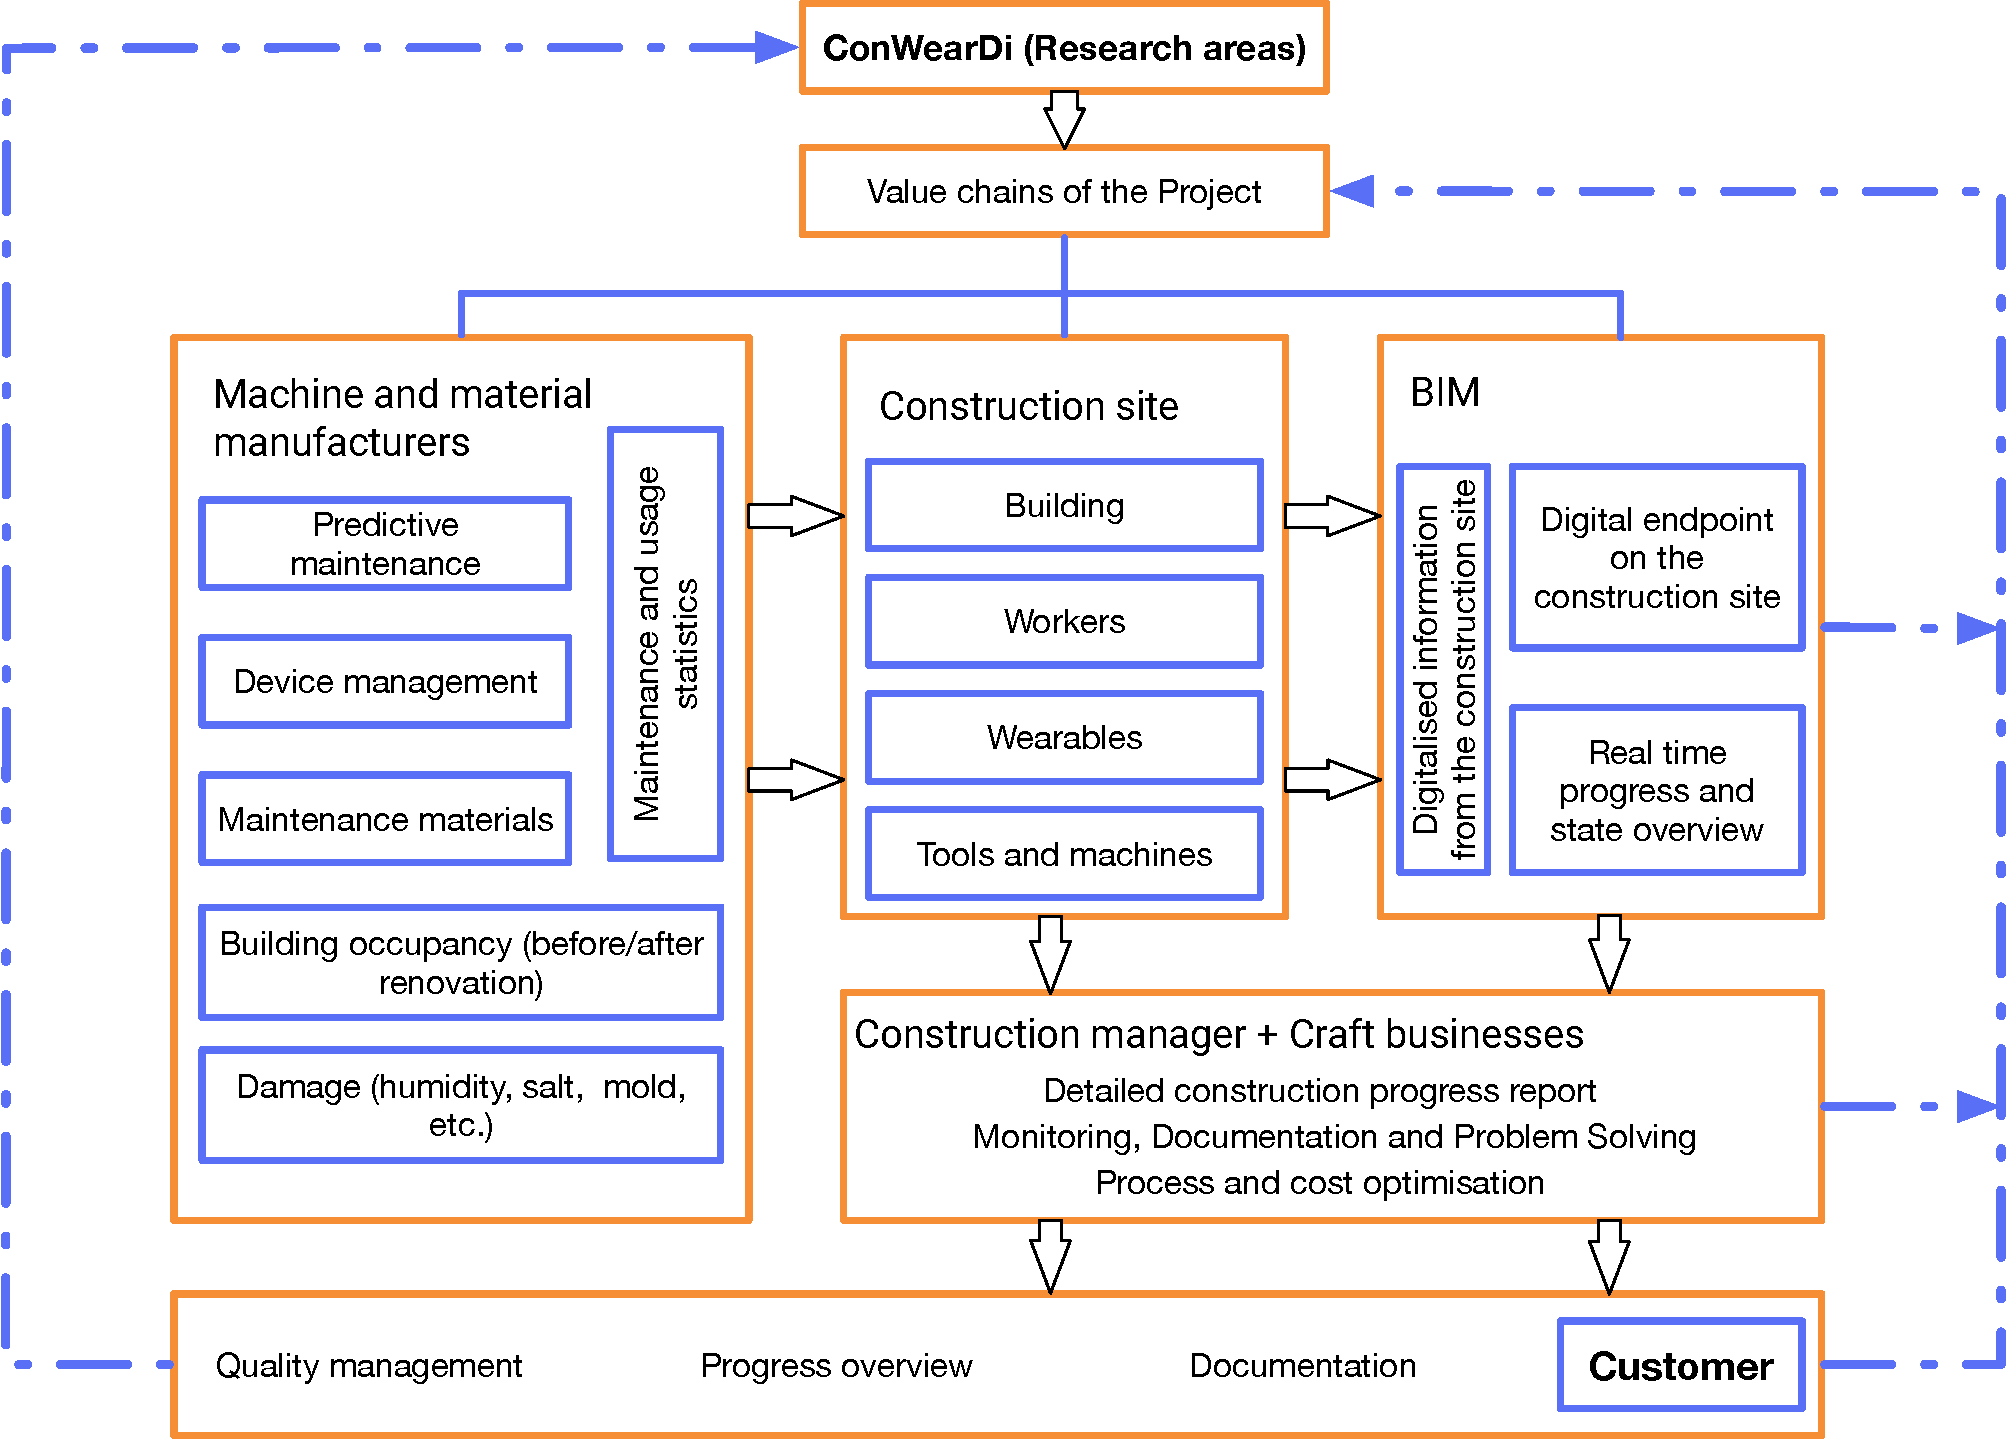
\includegraphics[width=0.8\textwidth]{figures/conweardi-functional.pdf}
\caption{Functional structure and main value chains of the ConWearDi project. The project tries to involve many stakeholders of the construction industry, such as machine manufacturers, construction workers, managers, etc. }
\label{fig:functional}
\end{figure*}

The most significant benefit, that we envision through realization of the ConWearDi system, is better efficiency in detecting and preventing problems and damages by improving or if possible fully automatizing construction site documentation and reporting workflows. 
Utilizing a real time information flow from the construction site, planners and managers are able to anticipate upcoming issues and avoid costly delays and damage repairs. 
Communication between customers, managers, designers and workers will also be improved by bundling of information such as agreements, used materials, tools and recorded working hours.
All in all, every stakeholder in the construction process will benefit from such a system. 
In the following paragraphs, we describe what new or improved services each participant of the process would be able to use during the execution of their role.


\subsection{Construction site manager}
Similar to industrial control processes, the construction site's current state would be available in real time through its digital twin.
This could help to recognize and avoid execution problems, e.g. when storage levels of the required materials are running low.
Auto-generated reports unload this time consuming task from the construction manager, and allow a more detailed documentation over time, saving the full history of the building creation.
This has major impact in later phases of construction or even in other phases of the building's life cycle, when previous decisions can be retraced and interface problems can be recognized. 

Continuous monitoring is also a powerful tool for the construction manager to fulfill his responsibilities about work safety and protecting the employees health. In a simple example, this can mean to prevent health risks caused by overtime or using heavy machinery without breaks and longer than allowed.
The accumulated knowledge can be used in other projects by learning from previous experiences (e.g. objective analysis of what went well, what went wrong).

\subsection{Designer and project coordinator}
Coordination processes can rely on digitally documented commitments instead of verbal agreements, since they are just as simple to create.
The project coordinator also benefits from the simplified, IT-supported trade-coordination based on the methods of Advanced Planning and Scheduling (APS).
Automatic documentation processes can be easily adapted later to support new standards and regulations, e.g. for fire safety.
The high resolution data can be fed into big data analytics services, e.g. to detect patterns across multiple construction projects which allows new possibilities to improve organizational processes.

\subsection{Machine and tool manufacturers, material suppliers}
For machine, tool and material producers or suppliers, the increased connectivity of their devices and their integration into the digital processes of their customers helps to better understand the market and customer behaviors. 
Based on the collected information, they are able to implement more efficient services and logistic coordination e.g. by predicting when the customer's material storage will be depleted.

Proactive maintenance services can be offered for construction site machines based on their usage and wear tracking. 
Furthermore, machine manufactures can adapt new business models which rely on the connectivity and information of sensor built into their machines. One example is just-in-time machine leasing, where customers pay only for the time during which the machine was actually used.

Material suppliers can offer proactive maintenance services for built-in materials by tracking their physical state and properties (e.g. temperature and humidity).
With the ever growing amount of collected sensor data and customer feedback, existing products can be improved and completely new solutions for the market can be developed and tested.


\subsection{Craftsman businesses and construction workers}
For craftsmen and workers on site, the connected system provides the possibility to easily access context related, reliable and up-to-date information. 
This will help ensuring execution quality and work safety by preventing mistakes caused by miscommunication. Moreover, this means fewer phone calls, less idle times and an overall streamlined and traceable information flow.

By using connected devices, manufactures are able to offer real time remote support services to help workers solving problems on site. A further reduction in costly down-times waiting for a replacement machine or a technician is to be expected.

Disruptions in processes can be reported by workers in an effortless manner, which with careful analysis could aid an organization in continuous optimization and improvement.

Real time target-performance measurement allows to avoid foreseeable delays via simulating and providing alternative solutions when needed. This leads to a generally optimized resource usage and a smart decision support system.


\section{Methodology}
The realization of the described vision is a complex task, even if many of the necessary subsystems exist and are currently used in other industries. 
Everything has to be adapted to the particular requirements and work culture of the construction industry and connected in a meaningful and realistic manner. 
The approach of the ConWearDi project for solving this task is to include experts from different professions and many different possible future stakeholders of the proposed system during all stages of research and development.
 
Figure \ref{fig:functional} shows the functional structure and main value chains of the ConWearDi project. Actual research questions will be aligned with the most important factors for the value chain until the end customer. 
The endpoints of the digital processes are moving towards the construction site, where the main execution of the construction process takes place.

To cover all necessary areas and ensure that all stakeholder groups are represented in the project, the consortium in ConWearDi actively involves:
\begin{itemize}
  \item J. Wagner GmbH - a company developing and producing construction machines, e.g. for airless spray painting - a commonly used tool in the building trade.
  \item DAW - among other things a manufacturer of isolation plates to be integrated into houses for better thermal efficiency.
  \item Sander + Partner GmbH - developer of ERP software for construction and craftsman businesses.
  \item a variety of multiple craftsman businesses with different grade of digitization.
\end{itemize}
Within the project, they work closely together with research groups from areas like cyber-physical systems and ubiquitous computing (DFKI\footnote{German Research Center for Artificial Intelligence}), process planning and optimization (Fraunhofer ITWM\footnote{Fraunhofer Institute for Industrial Mathematics} + eBZ\footnote{E-Business Competence Center, Planning and Construction}) and usability and psychological aspects of demands associated with the new technology (CCS, University of Kaiserslautern).

The first concrete implementation phase of the project explores equipping construction workers with different wearable devices to track working activities and support them with information through different output modalities.
Moreover deploying smart machines on construction sites, like spray painting machines extended with sensors and connectivity as well as smart materials, like isolation plates with integrated sensors are used to create data sets for insightful data analysis.

\section{Conclusion}
The ConWearDi project was started to showcase the potential of digitization in the construction industry and craftsman trade by designing and implementing demonstrators of novel services.
These services will help to significantly improve cost efficiency, reduce delays and increase overall quality of the construction work.
As a result, customer value and satisfaction, as well as productivity and employee satisfaction of the craftsman businesses will improve. 

More information about the project results and feedback from the pilot businesses will be posted on the project website: www.conweardi.de

\begin{acks}
  This work has been funded by the Federal Ministry of Education and Research of Germany (BMBF) within the framework of the project ConWearDi.
\end{acks}


\bibliographystyle{ACM-Reference-Format}
\bibliography{literature.bib}

\end{document}
